\documentclass[12pt]{article}
%\documentclass[12pt,preprint,nofootinbib]{revtex4-2}
%\documentclass[12pt,article,nofootinbib]{revtex4-2}

%\documentclass[final,5p,times,twocolumn]{elsarticle} 
%\documentclass{article}
\usepackage{graphicx} % Required for inserting images
\usepackage{epsfig}  
\usepackage{amssymb,amsmath}
\usepackage{tabularx}
\usepackage[table,xcdraw]{xcolor}
\usepackage{natbib}
\usepackage[greek,english]{babel}
\usepackage{caption}
\usepackage{float}
\captionsetup{skip=6pt}
\usepackage[font=small,labelfont=bf]{caption}
\usepackage{booktabs}
%\usepackage{ragged2e}
%\captionsetup{
%  justification=justified,
%  singlelinecheck=false
%}

\usepackage[colorlinks=true,linkcolor=blue,urlcolor=blue]
{hyperref}

\usepackage{svg}
% \usepackage{cite}

%% correct/editing packages
\usepackage[normalem]{ulem}
%\sout{Hello World}
\usepackage{soul}
% define a more "fluorescent" yellow -> \hl
\sethlcolor{yellow} % or: \sethlcolor{lime}
%\st{Hello world}
 

\newcommand{\red}{\textcolor{red}}
\newcommand{\blue}{\textcolor{blue}}
\newcommand{\G}{\color{teal}}

\begin{document}

\title{About the impact of the wealth-to-salary  ratio on economic inequality
}
\author{
Jhordan Silveira de Borba\thanks{sbjhordan@gmail.com}\\
Instituto de Física, Universidade Federal do Rio Grande do Sul,%Av. Bento Gonçalves 9500, Porto Alegre, 90560-001, Rio Grande do Sul, Brazil
\and
Sebastian Gonçalves\thanks{sebastiangoncalves@gmail.com}\\
Instituto de Física, Universidade Federal do Rio Grande do Sul%, Av. Bento Gonçalves 9500, Porto Alegre, 90560-001, RS, Brazil
\and
Celia Anteneodo \thanks{celia.fis@puc-rio.br}\\
Departmento de Física, PUC-Rio%, Rua Marquês de São Vicente 225 Gávea, Rio de Janeiro, 22451-900, Rio de Janeiro, Brazil
}


\date{\today}


\maketitle

\begin{abstract} 

In previous studies, using agent-based simulations of a model of a capitalist economy proposed by Ian Wright, we demonstrated that inequality in both wealth and income distributions is largely governed by a single key parameter: the ratio between average wealth per capita and the mean salary, denoted by $R$. This parameter captures the relative weight of accumulated assets with respect to labor income. Our results showed that larger values of $R$
systematically lead to higher levels of inequality, as measured by the Gini coefficient.
%
In the present work, we extend this analysis beyond the modeling framework and investigate whether this relationship holds in real-world economies. Using empirical data, we find strong evidence supporting the trend predicted by the simulations: economies characterized by higher values of $R$ tend to exhibit greater inequality. These findings suggest that $R$ provides a simple yet powerful macroscopic indicator linking structural economic conditions to observed inequality patterns.

\end{abstract}

 \section{Introduction} 
\label{sec:introduction}
Economic activity can be interpreted through the lens of complex systems, in which collective outcomes arise from  interactions among heterogeneous agents~\cite{JUSUP20221,yakovenko2009,Farmer2009}. Particularly within econophysics, this perspective has proven particularly useful for understanding robust empirical patterns, especially those associated with the distributions of income and wealth~\cite{yakovenko2009,shaikh}.  In this context, a range of agent based models (ABM), including random-asset exchange models~\cite{chatterjee2007econophysics,repec:spr:eurphb:v:73:y:2010:i:1:p:145-153} have been developed in the literature of econophysics. Among them, the Social Architecture of Capitalism (SA) model introduced by Ian Wright~\cite{WRIGHT2005589} provides a simple yet empirically grounded description of interactions between firms and workers, successfully capturing key stylized facts of wealth distributions, with a clear two-regime structure~\cite{dragulescu2001,yakovenko2023}.
%
In recent works~\cite{Borba2025,Borba2026}, we conducted a systematic exploration of the parameter space of the SA model and we identified a parameter governing the separation between the two regimes.
This parameter, denoted by $R$, is defined as the ratio of average wealth per capita to the mean wage. Our analysis shows that, in this model, the overall shape of the wealth distribution—including the emergence of a gap between classes, increasing concentration of wealth, and the disappearance of an intermediate stratum at high values of $R$ are largely determined by this ratio, with only minor sensitivity to system size. In particular, inequality, as measured by the Gini coefficient~\cite{PLATAPEREZ201579}, increases monotonically with $R$. 
Moreover these results are robust holding for realistic modifications of the original proposal~\cite{Borba2026}.

Motivated by these ABM results, we conduct an empirical assessment to examine whether the theoretical predictions are supported by real-world data. 
%
To this end, we construct  empirical estimates of $R$, using measures of average employee compensation and net personal wealth, drawing —among other sources— on data from the World Inequality Database (WID)~\cite{WID}. We find a positive relationship between $R$ and standard measures of inequality   for mature and advanced economies especially during periods known for the prevalence of liberal policies and stability, consistent with the model’s predictions.

Obtaining reliable data on income and wealth remains a significant challenge. Administrative regions often differ in how they define and measure these variables, and various organizations may employ distinct methodologies. Moreover, even within the same institution, methodological changes can occur over time. As a result, data are scarce for certain regions, and cross-comparisons between datasets compiled by different organizations are often nontrivial. These limitations are taken into account in the analysis and comparisons that follow. 

\section{Analysis of estimates of $R$ from real data} 
\label{sec:real}

We start by analyzing, in Section~\ref{sec:single}, the temporal evolution of the relationship between $R$ and the Gini coefficient within individual countries, focusing on the United States, France, and the United Kingdom.

In Section~\ref{sec:groups}, we extend the analysis from individual countries to a comparative study of groups of advanced economies using two different data sources.


\subsection{Individual countries}
\label{sec:single}

In the following analyses, unless otherwise stated, inequality is measured by the Gini coefficient of pre-tax national income\footnote{According to the WID definition, national income aims to measure the total income available to the residents of a given country~\cite{WIDglossario}.} and the Gini index of net personal wealth\footnote{According to the WID definition, net personal wealth corresponds to the total value of non-financial and financial assets held by households, minus their debts.}. To estimate $R$, we proxy $\overline{p}$  by average employee compensation\footnote{According to the WID definition, employee compensation corresponds to the total remuneration, in cash or in kind, paid by employers to employees in return for work done.} and we proxy $\overline{w}$  by net personal wealth, both expressed per adult individual and in local currency. All data are obtained from the World Inequality Database (WID)~\cite{WID}.

%%% \subsubsection{United States}

We first consider the United States (U.S.). Figure~\ref{fig:R-Real} shows the evolution of inequality in the U.S. from 1984 to 2021.
%
A clear positive relationship, as predicted by the model, is observed: increases in $R$ are associated with higher Gini coefficients for both income and wealth. Using Spearman’s rank correlation coefficient, we find a strong and statistically significant correlation between $R$ and income inequality ($\rho = 0.95$, $p < 0.05$).\footnote{Throughout the remainder of the text, all statistical analyses are assessed for statistical significance using a significance threshold of $p \leq 0.05$. For Spearman's rank correlation coefficient, statistical significance is evaluated using a permutation test.}  

 \begin{figure}[t!] 
     \centering
    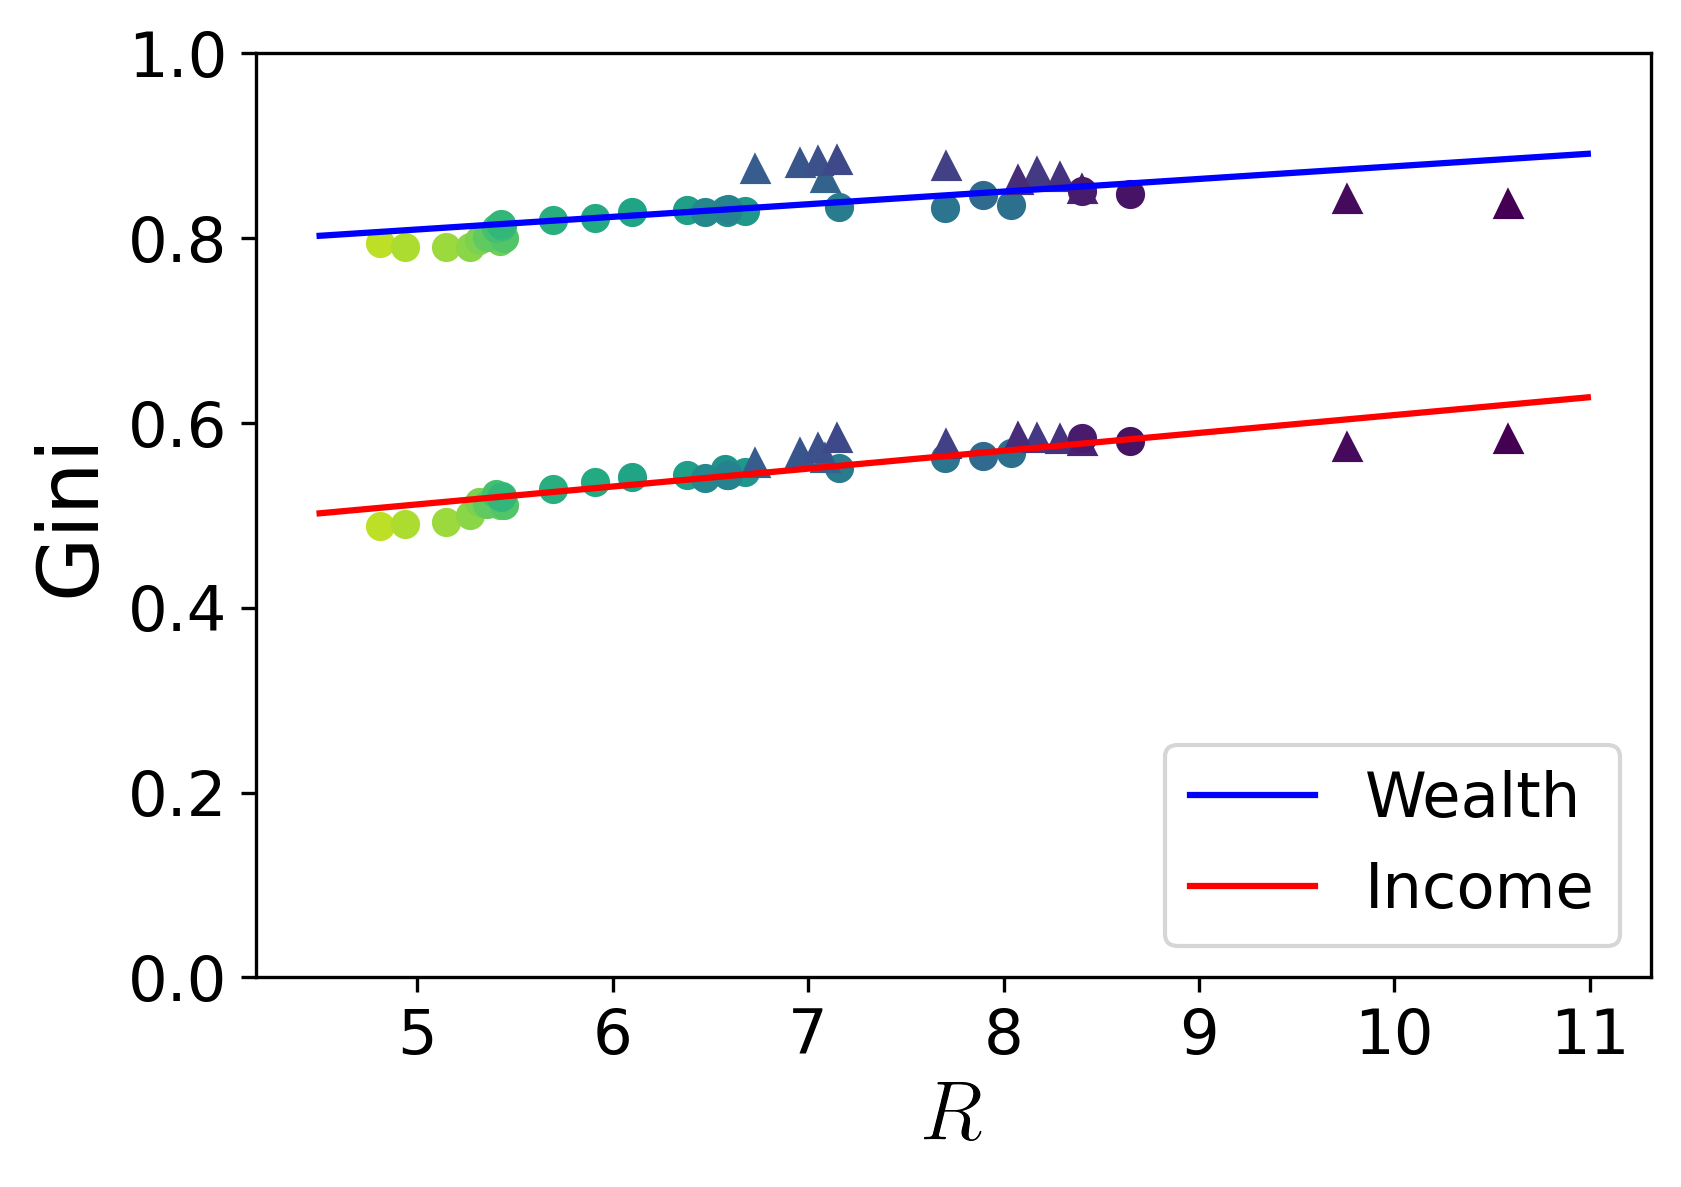
\includegraphics[width = 0.7\textwidth]{Figures/USA.png}
   
    \caption{United States: Gini indices for income and wealth vs. the $R$ ratio,   between 1984 and 2021, with the color gradient indicating the passage of time, from lightest (1984) to darkest (2021).  Triangle symbols highlight the years related to the ``Great Recession” (2008-2017) and COVID (2020) crises. Lines are linear regressions of the data. }
 \label{fig:R-Real}
\end{figure}

The analysis also yiedls a strong correlation $\rho = 0.83$ between inequality and $R$ as measured by the Gini coefficient for wealth,  which exhibits a similar qualitative pattern. In both cases, the two rightmost observations, marked with triangles and lying below the main trend,  correspond to the pandemic years (2020 and 2021). %% $p = 2 \times 10^{-4}$

For the Gini coefficient of wealth, several observations with $R$ close to 7 also deviate from the main trend.  These correspond to the decade following the onset of the 2008 financial crisis, known as the ``Great Recession''. More generally, the most atypical periods of the U.S. economy in this data set — the 2008 crisis and the 2020 pandemic — appear as departures from the overall trend.

It is worth noting that, although the crisis is typically dated from 2008 to 2009, its effects persisted for several years. For instance, as late as September 2015, full-time employment had not yet returned to its pre-crisis level~\cite{emprego-recessao}.\footnote{In absolute terms, the November 2007 level, 121,875 thousand, was only surpassed in October 2015, when it reached 122,094 thousand, without accounting for population growth.} Similarly, full-time employment in January 2022 had not yet recovered to its pre-pandemic level of 2019.\footnote{The December 2019 level, 131,675 thousand, had not yet been exceeded by January 2022, when it stood at 131,310 thousand.}

%\subsubsection{France}
Changes in the parameter $R$ and in the Gini coefficient reflect long-term dynamics. We therefore extend the analysis to the period from 1900 to 2015 for France\footnote{For France, wealth inequality data are missing for 1901, 1906, and 1908, while income inequality data are missing for 1901--1909 and 1911--1914.}, and the United Kingdom (U.K.)\footnote{For the United Kingdom, wealth Gini data between 1900 and 1980 are available only for the first year of each decade. For income inequality between 1900 and 2015, data are missing for 1907, 1909, 1915-1918, and 1942-1945.}, two countries for which relatively long and accessible time series are available.

  \begin{figure}[t!] 
 \centering
    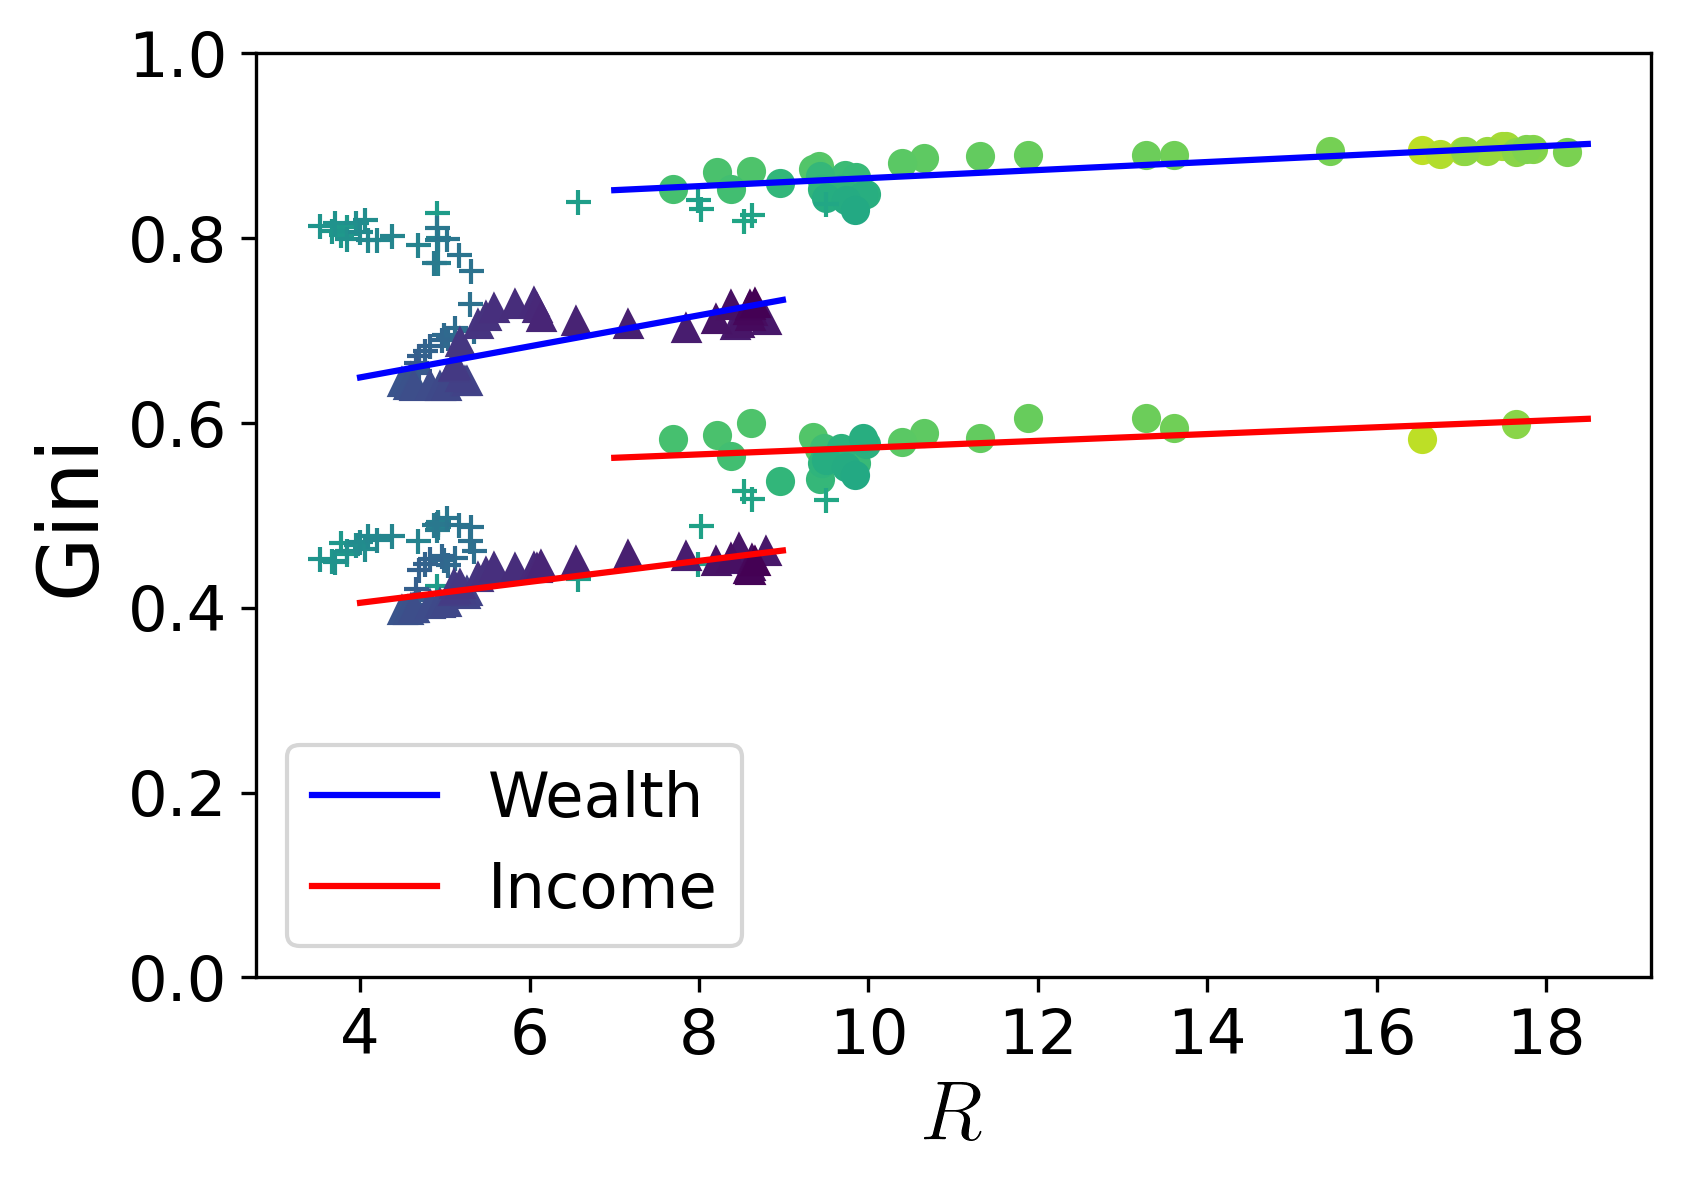
\includegraphics[width = 0.7\textwidth]{Figures/france.png}

    \caption{France: Gini indices for income and wealth vs. the $R$ ratio for France.   The data cover the period from 1900 to 2015, with the color gradient indicating the passage of time, from the lightest shades for the earliest years to the darkest shades for the most recent ones. Circles indicate data for the years between 1900 and 1929, where available, crosses symbols indicate observations from 1929 to 1980, while triangles indicate the period from 1980 to 2015. Trend lines were constructed for two periods, 1900--1929 and 1980--2015, whenever data were available.
}
 \label{fig:France}
\end{figure}

For France, in Fig.~\ref{fig:France}, we observe an increasing trend in inequality, measured either by the wealth Gini coefficient or by the income Gini coefficient, as $R$ increases, up to the 1930s.  This trend appears to re-emerge, with greater intensity, around the 1980s. Piketty argues that the tendency toward increasing inequality under capitalism was temporarily reversed between the two world wars and during the subsequent decades, a period marked by the expansion of the welfare state and the implementation of fiscal policies such as progressive taxation. According to this interpretation, the 1980s marked a return to policies associated with market deregulation~\cite{piketty}. This historical behavior is consistent with our findings.



% Belle Époque (1871-1914)  
% Guerras mundiais (1914-1945)
% Período de "welfare-state" (1945-1980)
% Ressurgimento do liberalismo (1980-atual)

%\subsubsection{United Kingdom}
Data from the United Kingdom, although scarcer, appear to exhibit the same trendm as we can observe in Fig.~\ref{fig:uk}. The historical trajectories of France and the United Kingdom, both of which played central roles in the development of capitalism, point to a relationship between the Gini coefficient and $R$, similar to the results found for the United States.

 \begin{figure}[h!] 
    \centering
    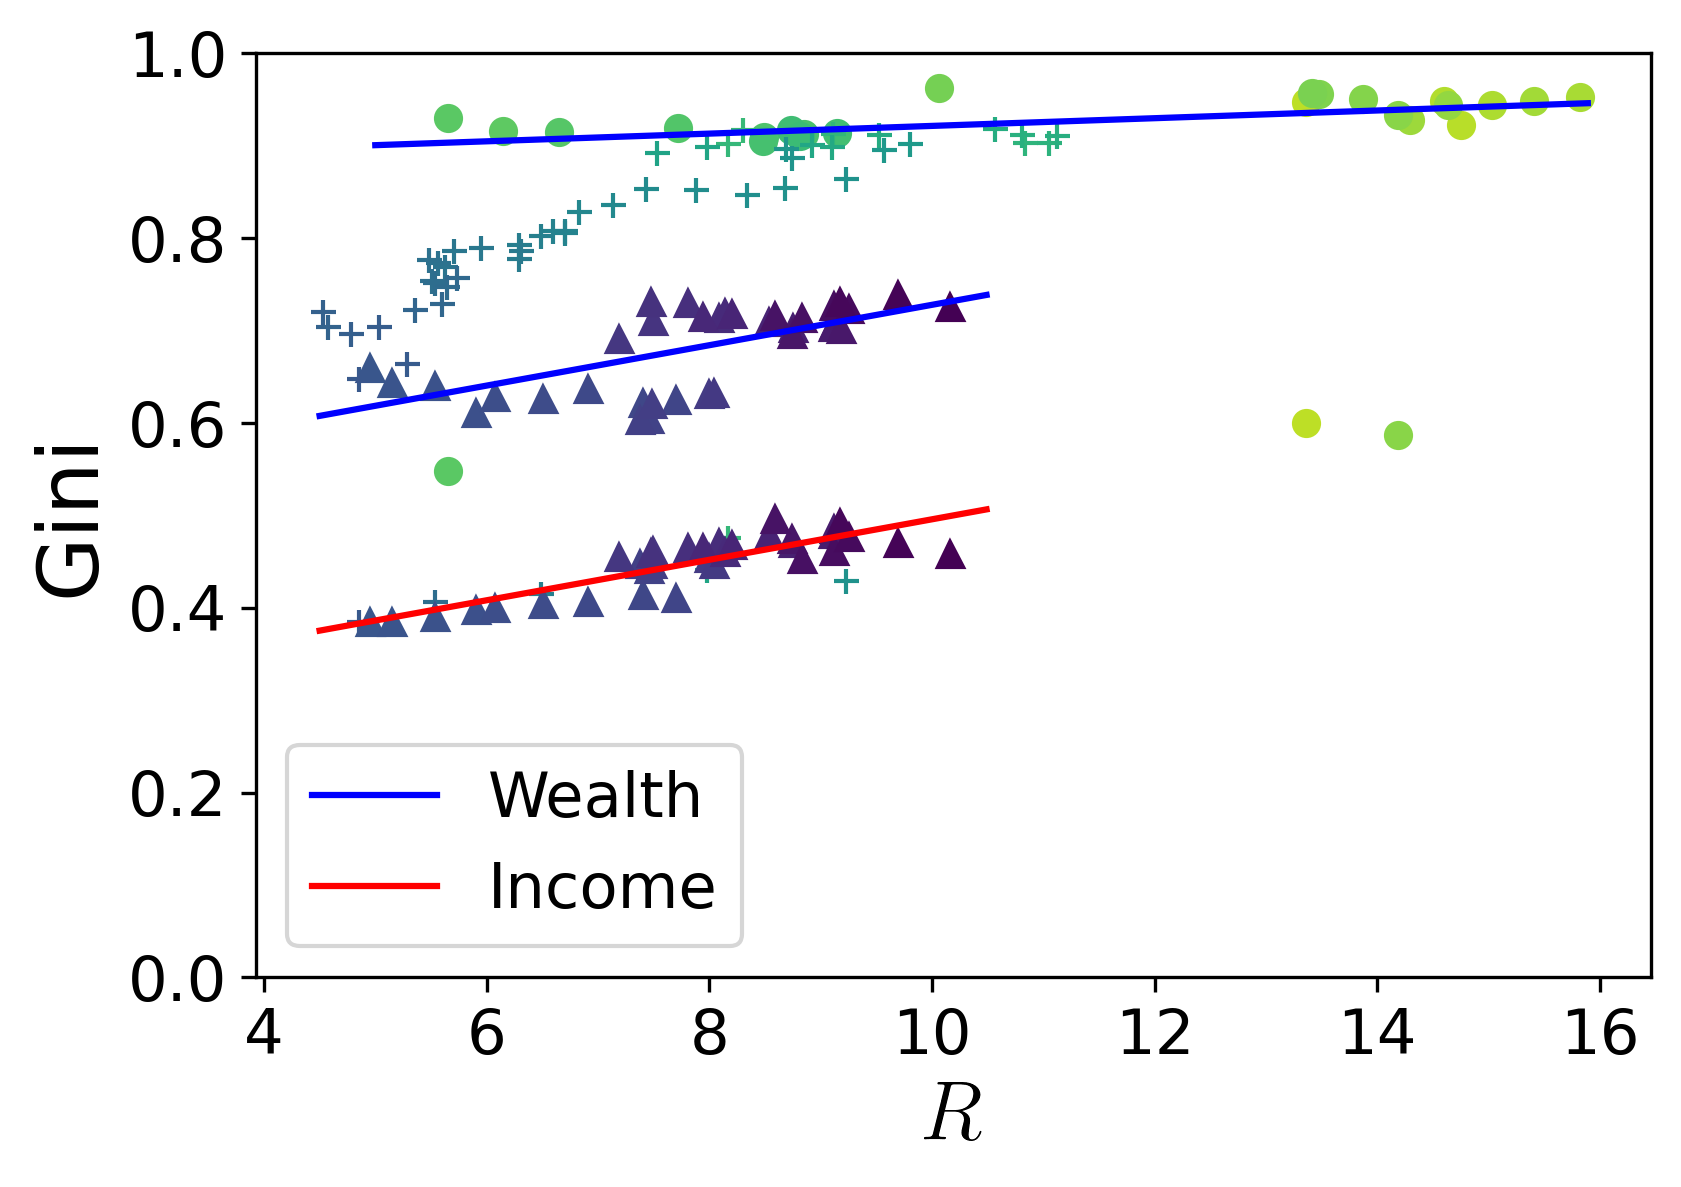
\includegraphics[width = 0.7\textwidth]{Figures/UK.png}
    \caption{United Kingdom: 
    Gini indices for income and wealth vs. the $R$ ratio. 
    The data cover the period from 1900 to 2015, with the color gradient indicating the passage of time, from the lightest shades for the earliest years to the darkest shades for the most recent ones. Circles indicate data for the years between 1900 and 1929, where available, crosses symbols indicate observations from 1929 to 1980, while triangles indicate the period from 1980 to 2015. Trend lines were constructed for two periods, 1900-1929 and 1980-2015, whenever data were available. Since there are virtually no U.K. income data for the first period, no corresponding trend line is shown.
}
 \label{fig:uk}
\end{figure}

These empirical results suggest that the behavior captured by the SA model reproduces key features of advanced market economies, in which high levels of inequality are not exceptional or crisis-induced, but instead emerge as a stable statistical property of the system. Periods of crisis, however, can be associated with deviations from this equilibrium, just as these dynamics can be influenced by government policies.

\subsection{Groups of  advanced economies}
\label{sec:groups}

For the analysis and comparison of groups of advanced economies, we consider two data sources:   the Organization for Economic Co-operation and Development (OECD)  and the World Inequality Database (WID).

\subsubsection{OECD data}

The OECD  is an important group in the contemporary global economy. To broaden the analysis and examine the relationship between $R$ and inequality across different country groups and databases, we extend the analysis to OECD countries using data provided by the OECD Data Explorer platform~\cite{OECD}.  We choose to do a cross-country comparison based on a five-year window, 2015--2019, chosen to exclude the pandemic period and focus on relatively stable economic conditions.

Ideally, such comparisons would rely on observations from the same year across countries, as well as multiple years for each economy. However, the frequency of the data provided by the platform makes this approach difficult. As an approximation, we define a time window and select, for each country, the most recent available observation within that window, while maintaining sufficient distance from the aftermath of the 2008 financial crisis. Despite this limitation, the dataset provides useful insight into the relationship between $R$ and the Gini coefficients across different countries within the same historical period.

Using this time window, and requiring that $\overline{w}$, $\overline{p}$, and the Gini coefficient refer to the same year for each country, the analysis included the 25 countries that had all the necessary data. The complete list of countries can be seen in the Table~\ref{tab:OECD}.

\begin{table}[]
\centering
\begin{tabular}{llllll}
Country & Year & \multicolumn{1}{l|}{Group} & Country & Year &  \\ \hline
Australia & 2018 & \multicolumn{1}{l|}{A} & Lithuania & 2016 & B\\
Austria & 2017 & \multicolumn{1}{l|}{A} & Luxembourg & 2018 & A\\
Canada & 2019 & \multicolumn{1}{l|}{A} & Netherlands & 2019 & A\\
Chile & 2017 & \multicolumn{1}{l|}{B} & New Zealand & 2018 & A\\
Denmark & 2019 & \multicolumn{1}{l|}{A} & Norway & 2018 & A\\
Estonia & 2017 & \multicolumn{1}{l|}{B} & Poland & 2016 & B\\
Finland & 2019 & \multicolumn{1}{l|}{A} & Portugal & 2017 & A\\
Germany & 2017 & \multicolumn{1}{l|}{A} & Slovenia & 2017 & B\\
Greece & 2018 & \multicolumn{1}{l|}{A} & Slovakia & 2017 & B\\
Hungary & 2017 & \multicolumn{1}{l|}{B} & Spain & 2018 & A\\
Ireland & 2018 & \multicolumn{1}{l|}{A} & United Kingdom & 2017 & A\\
Italy & 2016 & \multicolumn{1}{l|}{A} & United States & 2019 & A\\
Latvia & 2017 & \multicolumn{1}{l|}{B} &  &  & 
\end{tabular}
\caption{List of countries included in the OECD analysis, along with the year the data was collected and the group to which they belong. Group A consists of countries that were classified as advanced economies by the IMF in the 2000s, and Group B consists of the remaining countries.}
\label{tab:OECD}
\end{table}

In this analysis, $\overline{w}$ is proxied by net wealth per person,\footnote{According to the OECD definition, the concept of wealth used in the OECD Guidelines refers to ``ownership of economic capital'' as a dimension of people's material well-being.} measured at current prices.
%
The quantity $\overline{p}$ is proxied by the average annual wage,\footnote{According to the OECD definition, average annual wages per full-time equivalent dependent employee are obtained by dividing the national-accounts-based total wage bill by the average number of employees in the total economy, which is then converted into full-time equivalent units by applying the ratio of average usual weekly hours per full-time employee to those of all employees.} also expressed at current prices. Inequality is measured using the Gini coefficient of disposable income.\footnote{According to the OECD definition, the Gini coefficient is based on the comparison of cumulative proportions of the population against cumulative proportions of the income they receive and ranges from 0, in the case of perfect equality, to 1, in the case of perfect inequality.}

 Despite the challenges involved in cross-country comparisons, the data show a moderate tendency for inequality to increase as the parameter $R$ increases. Using Spearman's rank correlation, we obtain a coefficient $\rho=0.41$.%., with a statistically significant result ($p<0.05$).

We can hypothesize that, since our model seeks to model a purely capitalist economy, the observed trend in the relationship between the $R$ parameter and inequality is more pronounced in countries with more advanced economies that have been in place long enough to have reached a certain level of stability.

We therefore divide the countries into two groups.  Group A consists of 17 countries that were classified as advanced economies by the IMF at the beginning of the 2000s\cite{BackMatter},  and Group B consists of the remaining 8 countries\footnote{For Estonia, Latvia, Lithuania, Slovenia and Slovakia, the year in which each country joined the eurozone~\cite{eurozone} coincides with the year in which it began to be reported as an advanced economy, respectively: 2010, 2013, 2014, 2006 and 2008 \cite{FMI2010,FMI2013,FMI2014,FMI2008,FMI2006}.   This suggests that, for the International Monetary Fund, classification as an advanced economy depends not only on domestic economic indicators, but also on integration into a robust institutional and monetary bloc, such as the Eurozone. Chile, Poland, and Hungary are not considered advanced economies until the 2025 report~\cite{FMI2025}.}. 

The results can be seen in Figure   \ref{fig:R-OECD}. If we focus our analysis solely on the countries in Group A, the trend is noticeably more pronounced; when we repeat Spearman’s correlation test, the coefficient rises to $\rho=0.78$.



 \begin{figure}[h!] 
     \centering
    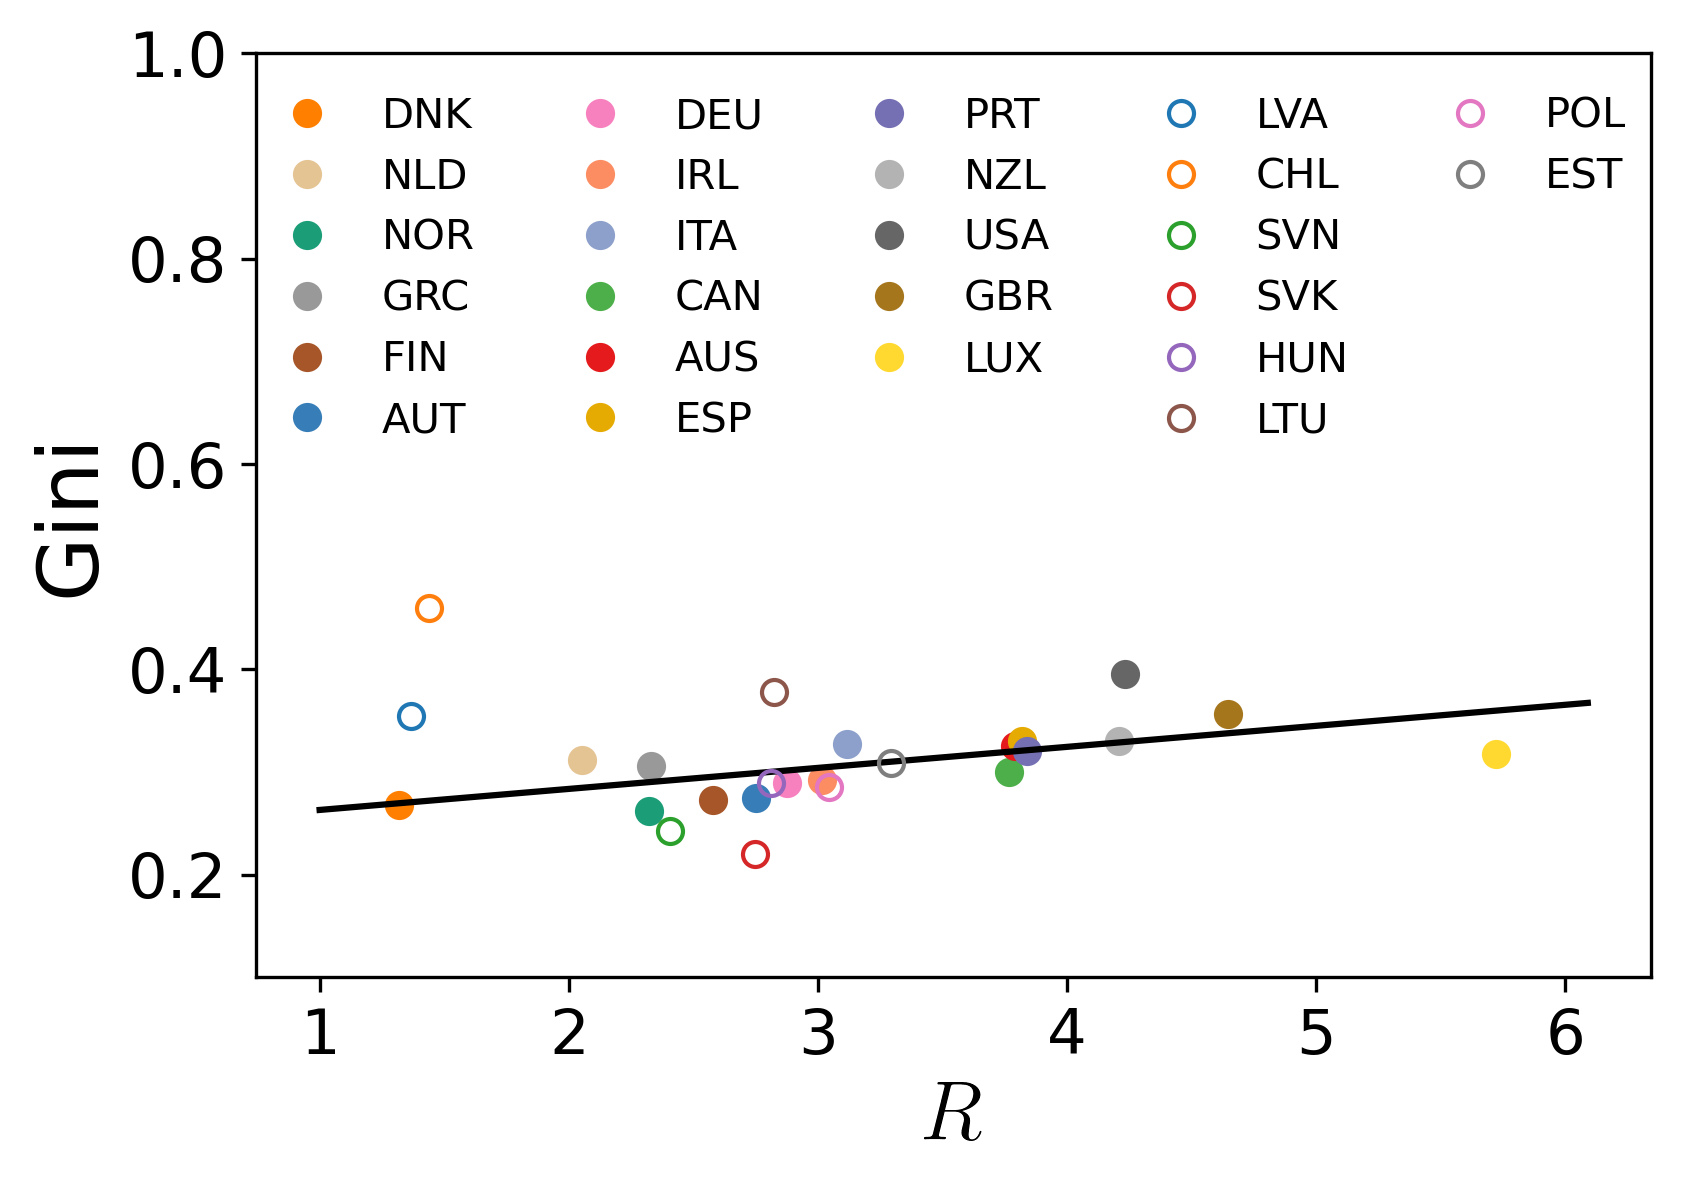
\includegraphics[width = 0.7\textwidth]{Figures/OECD.png}
    \caption{OECD countries: Income Gini index versus the $R$ factor, using the most recent data available within the period 2015-2019. Group A is shown with filled circles, and Group B with open circles.}
 \label{fig:R-OECD}
\end{figure}

So when we focus on more advanced and long-established economies, we observe a stronger and more statistically significant correlation between $R$ and inequality, as measured by the Gini coefficient. One way to interpret this result is through Erik Olin Wright’s conception of capitalism. According to Wright, to describe an economy as capitalist means that capitalist relations are the dominant relations within a given economic ecosystem, but not necessarily the only relations present in that economy~\cite{wright2022ser}.

Since the SA model represents a purely capitalist system, we may hypothesize that it better describes economies in which capitalist relations are more systematically institutionalized across social and economic life. This may explain why the model appears to fit more advanced and long-established capitalist economies more closely.

The SA model also describes a closed economy. In a globalized world, however, treating a country as a closed system may appear inconsistent with the realities of international economic integration. Ellen Meiksins Wood argues that national capitalist economies are interconnected and embedded in a global system governed by general capitalist laws, which bind capitalist economies together within a broader world economy~\cite{wood}.

Thomas Piketty shows that the net foreign wealth positions of most advanced economies have remained relatively small, often close to zero or slightly negative~\cite{piketty}. This suggests that external imbalances may not dominate domestic wealth dynamics in advanced economies, although non-advanced economies may behave differently.

To further investigate the role of international integration, we compute trade openness, defined as trade as a percentage of GDP.\footnote{World Bank definition: Trade is the sum of exports and imports of goods and services. This indicator is expressed as a percentage of Gross Domestic Product (GDP), which is the total income earned through the production of goods and services in an economic territory during an accounting period.} 

Using World Bank data for the years analyzed~\cite{WB}, when ranking the countries in the sample by trade openness, six of the nine most open economies belong to Group B, representing 75\% of that group. This suggests an association between greater trade openness and a more recent or less consolidated status as an advanced economy within our sample.

The two exceptions within Group B are Chile and Poland, which are still not classified as advanced economies. To put it another way, among the 9 countries with higher trade openness, the only 3 that belong to group A,  are Ireland, Luxembourg, and the Netherlands. These are also the only countries in the sample that appear among the top 10 in ``The world's biggest enablers of corporate tax abuse'' \cite{tax}, an index of corporate tax havens. This may introduce statistical distortions, since their trade-to-GDP ratios can be inflated by multinational profit-shifting and accounting practices. If these three countries are also excluded, the Spearman's rank coefficient increases to $\rho=0.90$.  The complete ranking is shown in Table \ref{table:all2}.

\begin{table}[h!]
\centering
\begin{tabular}{clc|clc}
Rank & Country                 & \% Tr. Op.   & Rank & Country        & \% Tr. Op.  \\
\hline
1       & Luxembourg$^{\dagger}$  & 361.9       & 14      & Greece         & 79.2        \\
2       & Ireland$^{\dagger}$     & 216.4       & 15      & Finland        & 79.1        \\
3       & Slovakia*               & 186.6       & 16      & Germany        & 77.6        \\
4       & Hungary*                & 165.0       & 17      & Norway         & 70.0        \\
5       & Netherlands$^{\dagger}$ & 160.7       & 18      & Spain          & 67.0        \\
6       & Slovenia*               & 158.7       & 19      & Canada         & 66.2        \\
7       & Estonia*                & 144.6       & 20      & U. Kingdom      & 63.1        \\
8       & Lithuania*              & 13.7        & 21      & Chile*          & 56.0        \\
9       & Latvia*                 & 128.7       & 22      & New Zealand     & 55.8      \\
10      & Denmark                 & 108.8       & 23      & Italy           &  54.4     \\
11      & Austria                 & 105.6       & 24      & Australia       & 43.7      \\
12      & Poland*                 & 96.9        & 25      & United States   &  26.3\\
13      & Portugal                & 84.8        &   &      &              
\end{tabular}
\caption{Ranking of countries by economic openness, measured as percentual trade openness. Countries belonging to group B are marked with an asterisk (*); and those belonging to group A have no marking, except for countries classified among the top ten tax havens, which are marked with a cross ($\dagger$).}
\label{table:all2}
\end{table}

Thus, countries with more open economies tend either to have a shorter history as advanced economies or to exhibit distortions associated with their role as tax havens. Taken together, these results suggest that a closed-economy model such as SA, despite its limitations, may approximate some structural features of large, mature capitalist economies that are less affected by extreme openness or accounting distortions.

\subsubsection{WID data}

Panel data analysis is a standard tool in econometrics and therefore provides a natural approach for testing the relationship between the parameter $R$ and inequality, as measured by the Gini coefficient, in empirical data.

We construct a balanced panel dataset in which all countries are observed in every year between 1995 and 2019. The end date is chosen to avoid the effects of the COVID-19 pandemic. The data are obtained from the WID, for countries classified as advanced economies by the IMF since 1995~\cite{imf1995weo}\footnote{Of the 23 countries listed as advanced economies, or industrialized economies in the terminology used at the time, Iceland was excluded due to lack of data. In addition to the 19 countries listed in Table~\ref{table:all}, the other three countries analyzed are Austria, Luxembourg, and Spain.}.

Since the original definition of $R$ in the SA model is based on averages computed over the entire population, the construction of a global indicator should account for differences in country population sizes. Otherwise, small economies would contribute with the same weight as highly populated countries, masking the differences in the relative size of national economies within the global economy.

For this reason, we calculate averages weighted by the employed population across countries \footnote{WID definition: Number of employed individuals.}.The average of national Gini coefficients is not mathematically equivalent to the Gini coefficient that would be obtained by merging all national populations into a single global distribution. Nevertheless, due to the difficulty in obtaining data for calculating the aggregate data, this represents a first attempt to account for population differences among countries. To keep the approach consistent, the average value of $R$ is calculated in the same way.

Taking yearly averages across all countries in the sample, we obtain Spearman correlation coefficients of $\rho=0.73$ for wealth inequality and $\rho=0.95$ for income inequality. The final result is shown in Fig.~\ref{fig:22countries}.

 \begin{figure}[h!] 
 \centering
    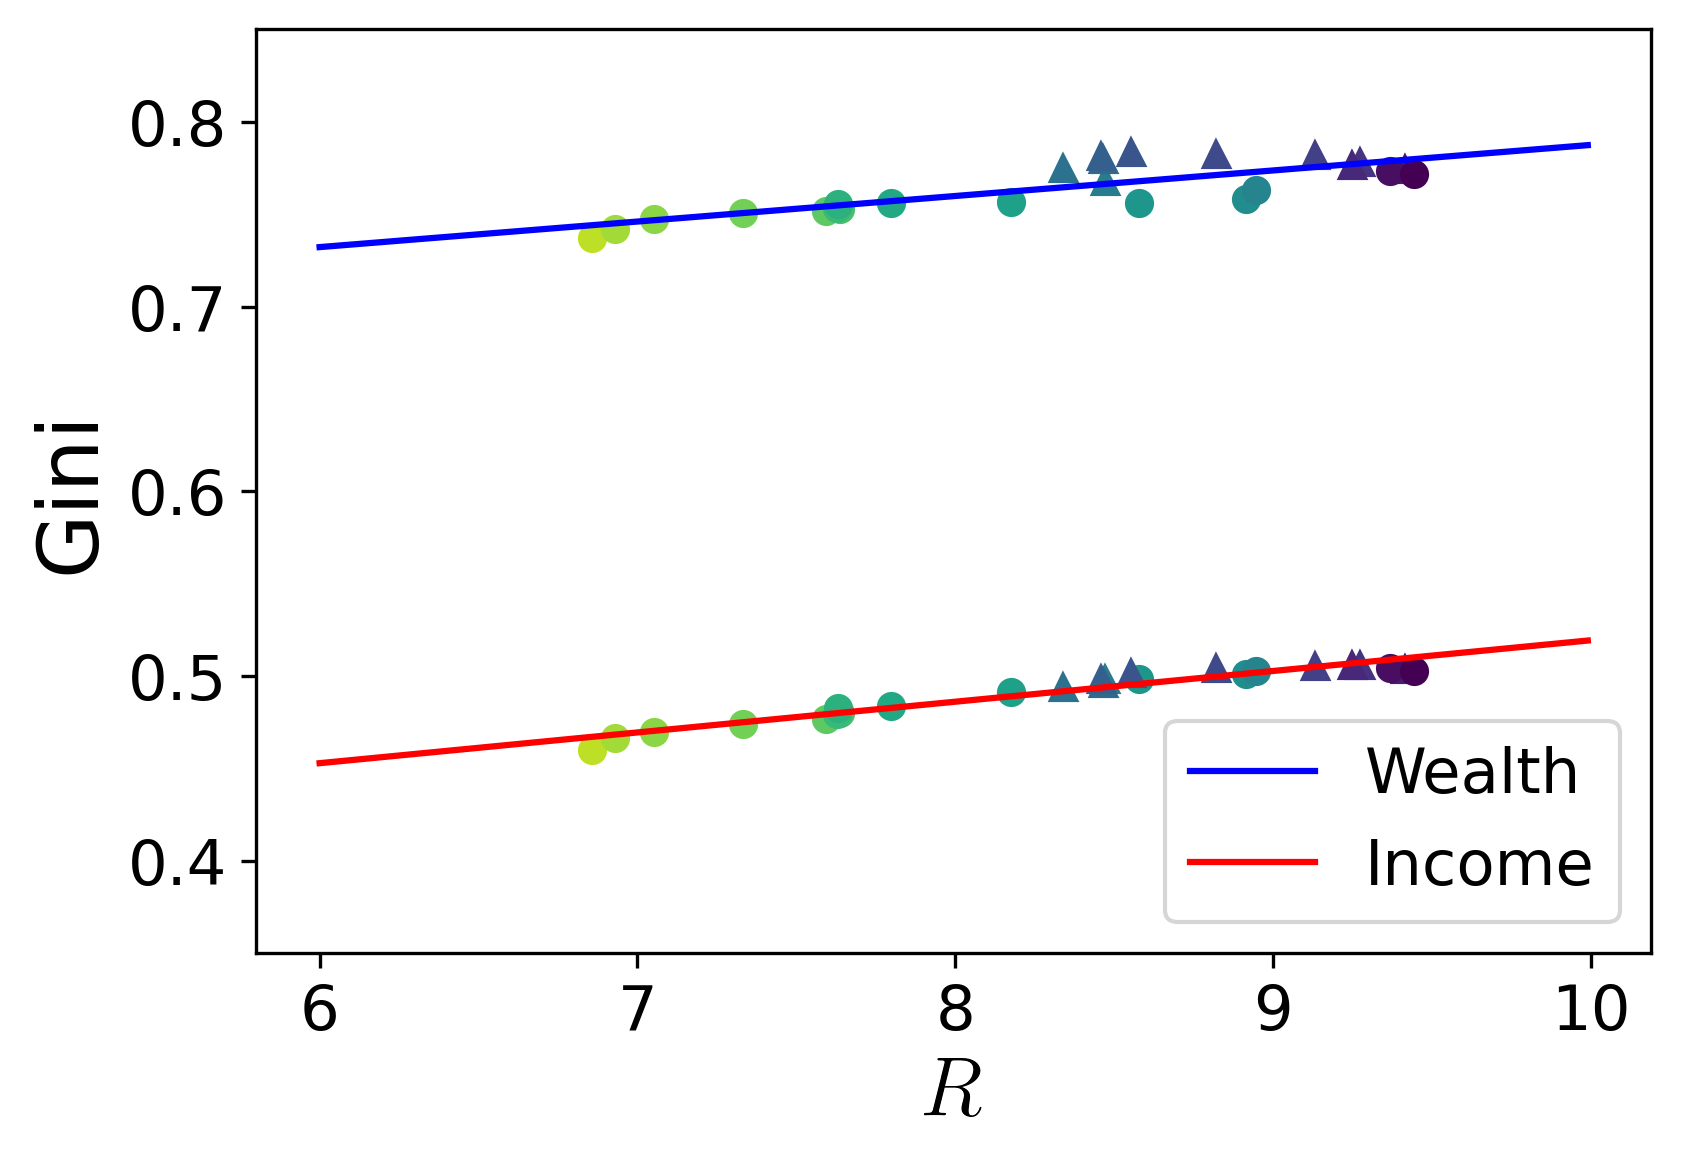
\includegraphics[width = 0.7\textwidth]{Figures/weighted.png}
    \caption{WID data: Relationship between $R$ and the Gini coefficients (income and wealth) for the population-weighted annual average of the 22 selected countries over a 25-year period.   With the marking in the star of the years related to ``Great Recession'' (2008-2017), the gradient color corresponds to the years, from the lightest (1995) to the darkest (2019).}
 \label{fig:22countries}
\end{figure}

Just as we discussed in the case of the U.S., we can see that the data for the decade following the Great Recession deviates from the trend line. What the analysis of this data indicates is the existence of a tendency for an increase in the ratio $R$ to be accompanied by an increase in inequality (both income and wealth) as measured by the Gini coefficient. 

Before proceeding, it is also worth making a few comments about the individual countries included in the dataset. Applying Spearman's rank correlation test individually to each country to examine the relationship between the  Gini coefficient and $R$ for the 22 countries in the sample. Excluding results that were not statistically significant, $82\%$ of the countries showed a positive correlation between $R$ and the Gini coefficient for income, and $72\%$ for wealth. These results are summarized in the Table ~\ref{table1}, which shows the absolute numbers.

\begin{table}[h!]
\centering
\begin{tabular}{lrr}
         & Wealth & Income \\
         \hline
Positive & 13& 14\\
Negative & 5      & 3      \\
Total    & 18& 17\end{tabular}
\caption{Summary of the analysis of signs of Spearman correlation for countries with statistically significant correlations. The entries indicate the number of countries showing a positive or negative correlation between $R$ and the Gini coefficient, separately for wealth and income inequality.
}
\label{table1}
\end{table}

It is noteworthy that 63\% of the countries that showed at least one statistically significant result\footnote{Of the 22 countries in total, 19 reported at least one significant result and 16 reported both.} did not show any negative correlation. This group includes several large advanced economies, including 6 of the world’s top ten largest by GDP in 2026, while the remaining 4 lie outside this study\cite{imfgpd}. The list of countries analyzed and their position in ranking by GDP size in current prices can be seen in the Table~\ref{table:all}. We can see that the first half of the ranking is dominated by countries that showed only a positive sign, and the second half is more populated by the other groups (mixed signals or only negative ones). 



\begin{table}[]
\centering
\begin{tabular}{clcclc}
Rank                   & Country        & \multicolumn{1}{c|}{GDP}  & Rank                 & Country         & GDP   \\ \hline
\textbf{1}             & United States  & \multicolumn{1}{c|}{32.4} & 11                   & Ireland         & 0.779 \\
2                      & Germany        & \multicolumn{1}{c|}{5.45} & 12                   & Belgium$^-$& 0.776 \\
3                      & Japan          & \multicolumn{1}{c|}{4.38} & 13                   & Sweden          & 0.760 \\
4                      & United Kingdom & \multicolumn{1}{c|}{4.26} & 14                   & Norway*         & 0.599 \\
5                      & France         & \multicolumn{1}{c|}{3.60} & 15                   & Denmark*        & 0.503 \\
6                      & Italy          & \multicolumn{1}{c|}{2.74} & 16                   & Portugal        & 0.380 \\
7                      & Canada*        & \multicolumn{1}{c|}{2.51} & 17                   & Finland         & 0.337 \\
8                      & Australia      & \multicolumn{1}{c|}{2.12} & 18                   & Greece*         & 0.307 \\
9                      & Netherlands*   & \multicolumn{1}{c|}{1.45} & 19                   & New Zealand$^-$& 0.278 \\
10                     & Switzerland    & \multicolumn{1}{c|}{1.15} & \multicolumn{1}{l}{} &                 &      
\end{tabular}
\caption{Ranking of the analyzed countries according to GDP (in thousands) in current prices. Countries with mixed correlation coefficients are indicated by an asterisk, and countries with only a negative sign are indicated by a minus sign. Countries that presented only positive coefficients do not receive any marking. }
\label{table:all}
\end{table}

The next step is to analyze the group of countries as a whole. To make proper use of panel data, before applying the Ordinary Least Squares regression technique we subtract the mean of each time series in order to reposition the distribution of points of all countries around the origin. In practice, this transformation removes the average level of each country and retains only the fluctuations around its own historical mean, corresponding to the econometric technique known as Fixed Effects.

In addition, it is interesting to take into account the distribution of the employed population across different countries obtained from WID.  In order to use population as a weight, Stata software requires a constant weight for each country. Therefore, we used the average population of each country calculated over the 25-year period analyzed. It should be noted that the ratio between the populations of the countries changed little during this period.  The country with the greatest absolute variation was the  U.S., the proportion of its population relative to the total population of the countries analyzed varied by less than 3\%, with maximum and minimum values of 33.81\% and 30.89\%, respectively. The same qualitative results were obtained when using any particular year as a reference, so we consider the average to be a good approximation.

Therefore, the contribution of each country to the minimization of residuals was weighted according to the fraction of workers represented by that country within the total working population of the sample. This corresponds to a weighted Fixed Effects analysis.

We choose this procedure, motivated by the objective of establishing a parsimonious baseline specification. Given the wide range of possible panel data approaches, we begin with a simpler framework. This baseline serves as a benchmark against which more demanding specifications can be evaluated. Specifically, it allows for a transparent evaluation of the relationship between $R$ and inequality before introducing additional layers of complexity.

We estimate a positive regression coefficient for both the income and wealth Gini coefficients. The coefficient is $\beta=8\times10^{-3}$ for wealth and $\beta=9\times10^{-3}$ for income, which corresponds to a change of near $~0.01$ of the Gini coefficient for each unit increase in $R$.   Given the relatively low temporal variability of Gini coefficients, even modest estimated effects may correspond to economically meaningful changes.  For example, when examining the variation in the global Gini coefficient for income (Purchasing Power parity - PPP) between 1980 and 2024, the maximum and minimum values are 0.86 and 0.83, respectively (if measured in Market Exchange Rates - MER, the values are 0.90 and 0.88). This corresponds to a maximum variation of only 0.03 (0.02) points over more than 40 years.

 \section{ Wealth-to-income ratio }
 
To the best of our knowledge, no studies in the economics literature investigate precisely the relationship between inequality and $R$. However, several works may contribute to the discussion. 
In Piketty’s terminology, the closest related quantity is $\beta$, the wealth-to-income ratio, rather than the wealth-to-wage ratio represented here by $R$. 
In a study by Piketty and Zucman, eight advanced economies are analyzed, and the authors concluded that in all these countries there has been a gradual increase in the wealth-income ratio in recent decades.  According to the authors, this increase is not necessarily problematic in itself, but it raises important questions concerning taxation and regulation, since high wealth-to-income ratios imply that wealth inequality is likely to play a central role in the overall structure of inequality in the twenty-first century~\cite{repec:oup:qjecon:v:129:y:2014:i:3:p:1255-1310}.
%https://gabriel-zucman.eu/files/PikettyZucman2014QJE.pdf

Madsen, on the other hand, focuses on the last eight centuries of British history and engages in critical dialogue with Piketty's work, but also concludes that the data suggest that variations in income inequality are accompanied by variations in $\beta$, i.e., the time series for income inequality follows a pattern very similar to that of $\beta$. The author further suggests that the wealth-to-income ratio may serve as a proxy for inequality \cite{MADSEN2019246}.

Given the documented relationship between inequality and $\beta$, it is useful to consider the relationship between $\beta$ and $R$, or, more specifically, between average income per capita and mean wages.  Although an increase in national income does not necessarily translate into an equivalent rise in mean wages, there is still a structural relationship between the two.  In aggregate terms, wages constitute a component of national income,  therefore, an expansion in national income may be expected to be associated with an increase in the average level of wages\cite{Przekota2023CausalityIT}.   

Thus, one may expect $\beta$ and $R$ to exhibit a qualitative long-run tendency,  insofar as average wages tend to increase with national income. In other words,  an increase in one tends to be accompanied by an increase in the other, albeit with different magnitudes, mediated by changes in the labor share ( the share of national income paid to workers as compensation), which determines how closely compensation dynamics track income growth.

Denoting the labor share by $s$ and national income by $Y$, a first approximation for the mean wage is $\overline{p}=sY/E$, where $E$ is the employed population. Defining the employment ratio as $\kappa=E/N$, where $N$ is the total population, and assuming that all labor compensation takes the form of wages, the average wealth is given by $\overline{w}=W/N$, where $W$ denotes total wealth. Under these assumptions, $R$ can be written as

\begin{equation}
   R = \frac{\overline{w}}{\overline{p}} = \frac{W/N}{s Y/E}=\frac{1}{s}\frac{W}{Y} \frac{E}{N}=\frac{\kappa}{s}\beta. 
\end{equation}
 
In other words, $R$ increases with $\beta$ when the labor share ($s$) and the employment ratio ($\kappa$) remain constant. Holding all other variables fixed, an increase in $\kappa$ also raises $R$. This is because keeping the total wage bill ($sY$) constant while increasing the number of employed workers reduces the mean wage. As a result, the relationship between $R$, unemployment, and inequality is nontrivial and may be non-monotonic, as explored in our recent work~\cite{Borba2026}, 
where we show that, according to the model, starting from a scenario of extremely high unemployment, increases in $R$ initially reduce inequality as both the mean wage and the unemployment rate decline. However, once unemployment reaches more realistic levels, the expected relationship emerges, with inequality increasing as $R$ continues to grow.

Data on the U.S. employment-population ratio over the past two decades (2006--2026) indicate remarkable stability throughout most of the period. Even during the 2008 financial crisis, it remained within the range of 58.3\% to 63.3\%. The main exception was the COVID-19 pandemic, when the ratio fell to 51.2\% in April 2020 before recovering to above 58.3\% by July 2021~\cite{taxa}.

Regarding the labor share, empirical studies suggest that this ratio has remained within a relatively narrow range, typically between 0.5 and 0.6, over long historical periods. This regularity is a well-known stylized fact in economics, often referred to as Bowley's law~\cite{farjoun2022labor}.

Analyzing a shorter time window, Karabarbounis and Neiman show that there has been a significant decline in labor share since the early 1980s, occurring mainly within the large majority of countries and industries~\cite{repec:nbr:nberwo:19136}. 
%
The Economic Policy Institute (EPI), analyzing the case of the United States, found positive annual growth in both productivity\footnote{According to the  Economic Policy Institute, productivity measures how much income is generated,
on average, in an hour of work. As productivity grows,  each hour of work generates more income over time. If productivity grows at a faster rate than compensation, 
this implies that a decreasing fraction of the income generated by labor is paid to workers as compensation, which is likely to reduce the labor share.}
%
and compensation (wages and benefits) paid per hour to workers, even though between 1979 and 2025 productivity grew at an annual rate of 1.6\% while compensation grew by only 0.6\%\cite{epi_productivity_pay_gap_2026}, widening the inequality\footnote{There are some challenges to these findings, such as the debate raised by the conservative think tank American Enterprise Institute (AEI) regarding the methodological choices adopted by the EPI. However, what the institute argues is that compensation growth has kept pace with productivity growth, not that it has outpaced it. Therefore, this does not undermine our analysis\cite{AEI}. }.

However, this does not contradict our findings. Positive growth in $\beta$ is still related to positive growth in $R$. 
Moreover, differences in growth rates arising from changes in the labor share over recent decades may have contributed to increasing inequality and are reflected in the behavior of $R$. Thus, our analysis of the parameter $R$ finds indirect support in the existing literature.
 
\section{Final remarks and conclusion}
\label{sec:final}

The results for the three countries analyzed here, together with those from the subsequent cross-country analysis, suggest that the model better captures the dynamics of advanced capitalist economies that are institutionally stable and economically mature. Deviations from the main trend appear to be associated with atypical economic periods, such as crises, stronger dependence on international markets, or lower levels of economic development.

An interesting direction for future research would be to  test whether these patterns hold at the global level. When considering the world economy as a whole, it must necessarily be treated as a closed system. However, this task faces the challenge of obtaining reliable data that accurately reflect the state of the global economy.

To conclude, it is useful to return to a classical insight that remains directly relevant to the present analysis. As Adam Smith wrote in The Wealth of Nations:
``No society can surely be flourishing and happy, of which the far greater part of the members are poor and miserable. It is but equity, besides, that they who feed, clothe, and lodge the whole body of the people, should have such a share of the produce of their own labor as to be themselves tolerably well fed, clothed, and lodged.''~\cite{smith1776wealth} 

 

{\bf Acknowledgments:}
We acknowledge financial support from CAPES (Fundação Coordenação de Aperfeiçoamento de Pessoal de Nível Superior), through finance code 001, 
and CNPq (Conselho Nacional de Desenvolvimento Científico e Tecnológico) for Universal 406820/2025-2. 
C.A. also acknowledges partial financial support from CNPq for grant 308347/2025-0) and FAPERJ (Fundação de Amparo à Pesquisa do Estado do Rio de Janeiro), for CNE E-26/204.130/2024. S.G. would also like to thank CNPq for partially supporting this work under grant 309560/2025-0.

%\bibliographystyle{plainnat}
%\bibliographystyle{unsrt}
\bibliographystyle{plain}
\bibliography{referencias}


 
\end{document}